%%%%%%%%%%%%%%%%%%%%%%% file template.tex %%%%%%%%%%%%%%%%%%%%%%%%%
%
% This is a template file for Web of Conferences Journal
%
% Copy it to a new file with a new name and use it as the basis
% for your article
%
%%%%%%%%%%%%%%%%%%%%%%%%%% EDP Science %%%%%%%%%%%%%%%%%%%%%%%%%%%%
%
%%%\documentclass[option]{webofc}
%%% "twocolumn" for typesetting an article in two columns format (default one column)
%
\documentclass{webofc}
\usepackage[varg]{txfonts}   % Web of Conferences font
%
% Put here some packages required or/and some personnal commands
%
%
\begin{document}
%
\title{ServiceX}
%
% subtitle is optionnal
%
\subtitle{A Distributed, Caching, Columnar Data Delivery Service}

\author{\firstname{B.} \lastname{Galewsky}\inst{1}\fnsep\thanks{\email{bengal1@illinois.edu}} \and
        \firstname{R.} \lastname{Gardner}\inst{2}\fnsep\thanks{\email{rwg@uchicago.edu}} \and
        \firstname{L.} \lastname{Gray}\inst{5}\fnsep\thanks{\email{Lindsey.Gray@cern.ch}} \and
        \firstname{M.} \lastname{Neubauer}\inst{1}\fnsep\thanks{\email{msn@illinois.edu}} \and
        \firstname{J.} \lastname{Pivarski}\inst{3}\fnsep\thanks{\email{pivarski@princeton.edu}} \and
        \firstname{M.} \lastname{Proffitt}\inst{4}\fnsep\thanks{\email{masonlp@uw.edu}} \and
        \firstname{I.} \lastname{Vukotic}\inst{2}\fnsep\thanks{\email{ivukotic@uchicago.edu}} \and
        \firstname{G.} \lastname{Watts}\inst{4}\fnsep\thanks{\email{gwatts@uw.edu}} \and
        \firstname{M.} \lastname{Weinberg}\inst{2}\fnsep\thanks{\email{mweinberg@uchicago.edu}}
}

\institute{University of Illinois at Urbana-Champaign
\and
           The University of Chicago
\and
           Princeton University
\and
           University of Washington
\and
           Fermilab
          }

\abstract{%
  We will describe a component of the Intelligent Data Delivery Service being developed in
  collaboration with IRIS-HEP and the LHC experiments. ServiceX is an experiment-agnostic service
  to enable on-demand data delivery specifically tailored for nearly-interactive vectorized
  analysis. This work is motivated by the data engineering challenges posed by HL-LHC data volumes
  and the increasing popularity of python and Spark-based analysis workflows.
  \medskip
  
  ServiceX gives analyzers the ability to query events by dataset metadata. It uses containerized
  transformations to extract just the data required for the analysis. This operation is collocated
  with the data lake to avoid transferring unnecessary branches over the WAN. Simple filtering
  operations are supported to further reduce the amount of data transferred.
  \medskip
  
  Transformed events are cached in a columnar datastore to accelerate delivery of subsequent
  similar requests. ServiceX will learn commonly related columns and automatically include them in
  the transformation to increase the potential for cache hits by other users.
  \medskip
  
  Selected events are streamed to the analysis system using an efficient wire protocol that can be
  readily consumed by a variety of computational frameworks. This reduces time-to-insight for
  physics analysis by delegating to ServiceX the complexity of event selection, slimming,
  reformatting, and streaming.
}
%
\maketitle
%
\section{Introduction}
\label{sec:intro}
Data organization in HEP experiments often follows a standard workflow, starting from raw detector
data or simulated data, which is processed by reconstruction algorithms into higher-level physics
objects. This reconstructed data is stored in ROOT files in a nested branch structure and used as
input to analysis software to produce physics insights. While the reconstruction step is typically
performed centrally and a standardized output is made available to the entire collaboration, the
analysis software is often written by small groups or individual analysts, with idiosyncratic
selection and processing steps.

This approach carries with it a number of issues. Because transmission of reconstructed ROOT files
via wide area network is expensive, the analysis step must often be performed via jobs running on
the grid, which involve substantial overhead and require care and attention from the user. Further,
the output of these jobs is immutable, so changes to the analysis structure often require rerunning
the analysis code from scratch. Lastly, the format itself can impose barriers to insight: too much
craft is required to extract features (e.g. for ML applications) and the tools required to interact
with ROOT files are not generally transferable to other formats.

\section{ServiceX overview}
\label{sec:overview}

ServiceX, a part of the IRIS-HEP Data Organization, Management, and Access (DOMA) effort, is an
experiment-agnostic service that seeks to address these problems by enabling on-demand data
delivery, specifically tailored for nearly-interactive, high performance array-based and Pythonic
analyses. It provides uniform backend interfaces to data storage services and frontend
(client-facing) service endpoints for multiple different data formats and organizational
structures.

It is capable of retrieving and delivering data from data lakes, using Rucio to find and access the
data. The service is capable of on-the-fly data transformations to enable data delivery in a
variety of different columnar formats, including small flat ROOT files and streaming Apache Arrow
buffers. In addition, ServiceX includes pre-processing functionality for event data and preparation
for clustering frameworks (e.g. Apache Spark). Eventually, it will be able to automatically unpack
compressed formats, potentially using hardware accelerated techniques, and will prefilter events so
that only useful data is transmitted to the user.

\subsection{ServiceX features}
\label{subsec:features}
% Don't forget to give each section, subsection, subsubsection, and paragraph a unique label (see Sect.~\ref{sec:overview}).

ServiceX orchestrates containerized experiment-approved frameworks in order to produce data in
columnar formats. It includes a REST server interface that can be colocated with the data lake and
can easily be deployed to a local Tier 3 cluster. The service supports simple event selection to
enable users to extract only required subsets of data, and streams the output to analysis code in
the form of uproot-based awkward arrays \cite{uproot}.

This output is managed by the Kafka \cite{RefEventStreams} message broker, illustrated in
figure~\ref{fig:kafka}. The message broker caches results in order to make them available for
instant replay so output can be quickly analyzed and reanalyzed multiple times.

\begin{figure}[ht]
  \centering
  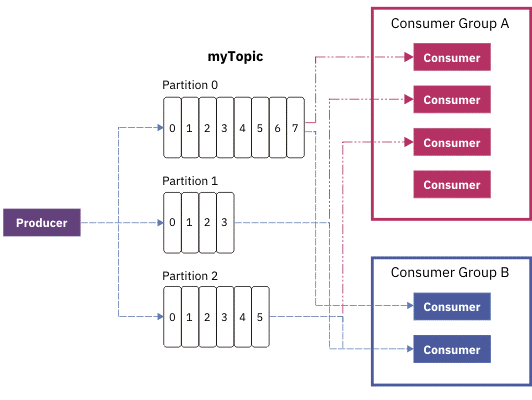
\includegraphics[width=0.75\textwidth]{kafka}
  \caption{Kafka uses a fault-tolerant, low-latency publish-subscribe messaging system.}
  \label{fig:kafka}
\end{figure}

The service is also capable of using Object Store to manage the output as a series flat ntuples
stored inside small ROOT files or HDF5 files. This effectively allows ServiceX to provide an
``ntuples-as-a-service'' functionality.

Finally, ServiceX is designed to be completely transactional, allowing data in the request to be
processed in parallel while ensuring all data is processed exactly once. This means there is no
danger of missed or double-counted events, even in the event of failure of one of the
transformation threads.

\subsection{Simple transform requests}
\label{subsec:requests}

An example transform request is presented below for illustration:

\bigskip

{\raggedright \footnotesize
  \texttt{\{}
  
  \texttt{"did": "mc15\_13TeV:mc15\_13TeV.361106.PowhegPythia8EvtGen\_AZNLOCTEQ6L1\_Zee.merge",}
  
  \texttt{"columns": "Electrons.pt(), Electrons.eta(), Muons.eta(), Muons.phi(), Muons.e()",}
  
  \texttt{"image": "sslhep/servicex-transformer:v0.1",}
  
  \texttt{"result-destination": "kafka",}
  
  \texttt{"kafka":\{}
  
  \texttt{    "broker": "servicex-kafka-1.slateci.net:19092"}
  
  \texttt{\},}
  
  \texttt{"chunk-size": 9000,}
  
  \texttt{"workers": 17}
  
  \texttt{\}}
}

\bigskip

Here the \texttt{did} field gives the ID of the dataset in Rucio, while \texttt{columns} gives the
list of columns requested by the user. The \texttt{image} field has the versioned image to be used
for the transformation. This piece can be easily swapped out for different transformers in order to
transform input files with different formats. Next the request specifies the Kafka broker to which
the output will be assigned. The last two fields indicate that each message in the Kafka topic will
contain 9000 events, and a total of 17 transformers will be spun up to process the dataset.

The output of this transformation request arrives as an Arrow table comprising 147,000 rows (one
for each event in the dataset) and 8 columns (corresponding to the attributes specified in the
request). Each entry contains an array whose length is the number of particles (i.e. electrons or
muons) in the event. The output is intended to work seamlessly with the uproot framework.

\section{ServiceX implementation}
\label{sec:implement}

\subsection{ServiceX architecture}
\label{subsec:architect}

The current architecture employed in ServiceX is illustrated in figure~\ref{fig:architectureV1}.
The service relies on a number of interconnected microservices which communicate via the REST
server. The DID finder is responsible for querying Rucio for the location and metadata of the files
in the user request. The preflight check then takes this information and performs some preliminary
transformations to verify the request is properly formed (e.g. refers to an existing dataset and
requests columns that can be found in the files). The transform manager is responsible for spinning
up the appropriate number of transformers to transform the dataset, and ensures that each file is
claimed by exactly one transformer. Finally, the transformer itself is responsible for converting
the input format into the requested output.

% Here we should perhaps have more description concerning the role of RabbitMQ, Minio and Kafka,
% and perhaps the role k8s plays in orchestrating the various pieces.

\begin{figure}[ht]
  \centering
  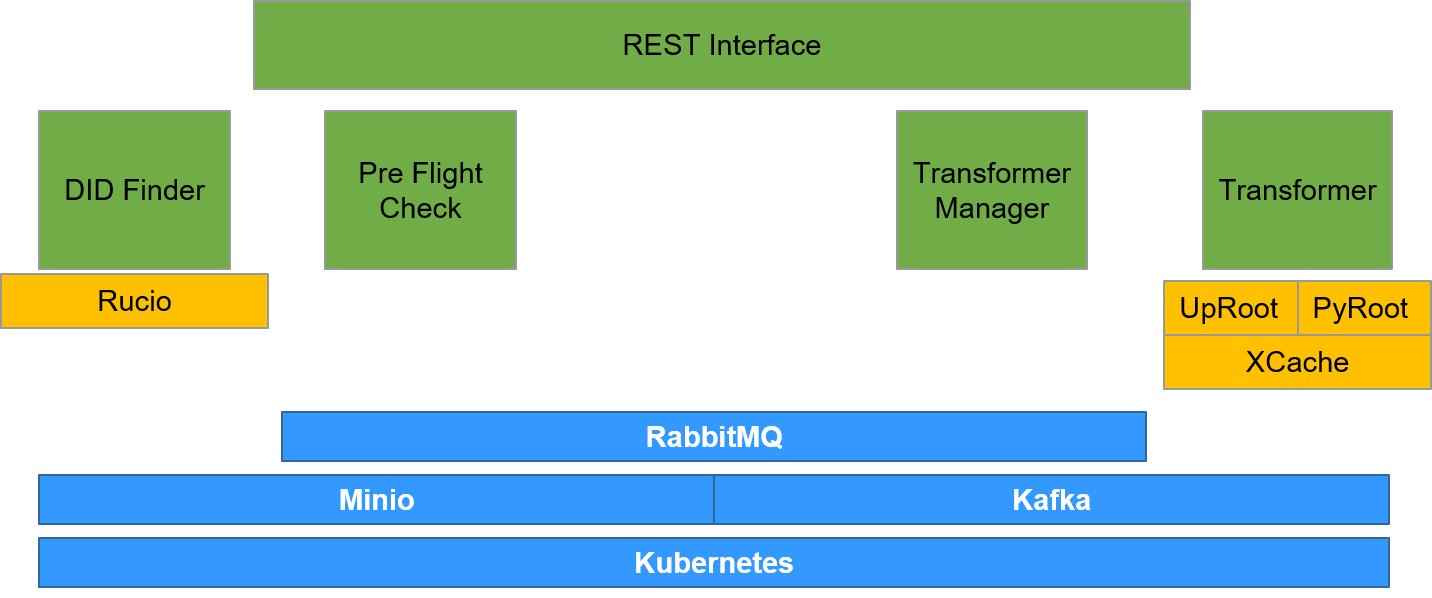
\includegraphics[width=0.75\textwidth]{architectureV1}
  \caption{Architecture for ServiceX version 1.}
  \label{fig:architectureV1}
\end{figure}

\subsection{Python transformers}
\label{subsec:pyTransform}

The transformers are the engine of the service, responsible for changing the format of the input
files into an analysis-friendly columnar output and sending this output to the message broker.

There are currently images available for transformers compatible with two different input formats.
First there is a transformer for the ATLAS xAOD/DAOD reconstruction format, based on the ATLAS
Analysis Base software. It employs pyROOT to access individual branches, and requires the use of
\texttt{for} loops due to the embedded data structures. The transformer has some limitations: the
need to loop over events in pyROOT makes the transformation quite slow, and the format contains no
information about the calibrated physics objects. Further, filtering is not yet implemented in this
transformer.

The second available transformer can handle ROOT files containing flat trees (i.e. trees whose
branches are all simple arrays). This makes them appropriate both for typical end-stage analysis
ntuples and for the CMS nanoAOD format, which features this flat tree structure. Here the
transformation can be performed directly with uproot tools, so the process is much faster. This
transformer also does not currently have in-place filtering implemented.

% \begin{figure}[ht]
%   \centering
%   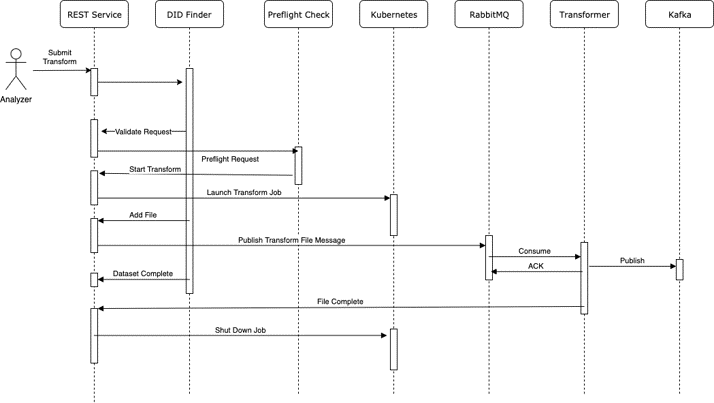
\includegraphics[width=0.75\textwidth]{sequenceDiagram}
%   \caption{Sequence diagram showing information flow in ServiceX.}
%   \label{fig:sequenceDiagram}
% \end{figure}

\section{What's next?}
\label{sec:whatNext}

ServiceX is being developed as an open source project intended to meet a broad range of analysis
needs within HEP. Consequently we welcome involvement from the HEP community. Version 1 is
available today and can be found at \cite{RefServiceX}. It builds on an extensive ecosystem of
open-source technologies, shown in figure~\ref{fig:openSourceTech}. We invite users to try out the
ServiceX demo and to reach out to us about providing data for your analysis.

\begin{figure}[ht]
  \centering
  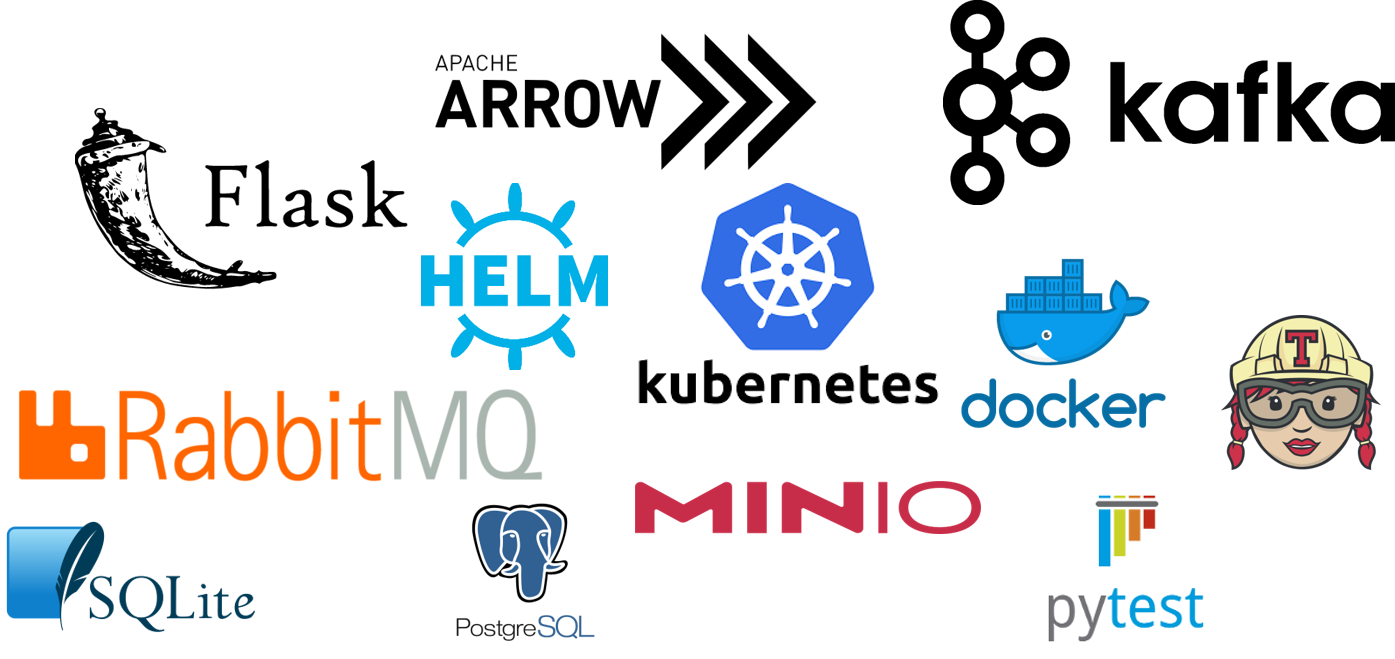
\includegraphics[width=0.75\textwidth]{openSourceTech}
  \caption{Multiple open-source technologies were used in the development of ServiceX.}
  \label{fig:openSourceTech}
\end{figure}

In addition, the project features many exciting new developments, including the use of very fast
C++ transformers and the implementation of a selection language to enable in-place filtering. Those
who are interested are encouraged to join the discussion on new features, and to help build
ServiceX!

\subsection{Version 2--with C++ transformers}
\label{subsec:v2}

ServiceX version 2 will feature transformers based on C++ code, and will be available in January
2020. This version will accept SQL-like selection statements specifying requested output columns as
well as filtering requirements, and will also enable the implementation of experiment-specific
calibrations on the raw physics objects. The architecture for this version of ServiceX will differ
slightly from the current architecture in the addition of the code generator service, which is
responsible for converting these statements into compiled C++ code and passing this to the
transformation manager (see figure~\ref{fig:architectureV2}).

In the case of the ATLAS xAOD format, this will enable the transformers to use ATLAS-specific code
running in the EventLoop framework. They will perform the transformations much faster than the
current implementation, and will have access to the calibration information.

\begin{figure}[ht]
  \centering
  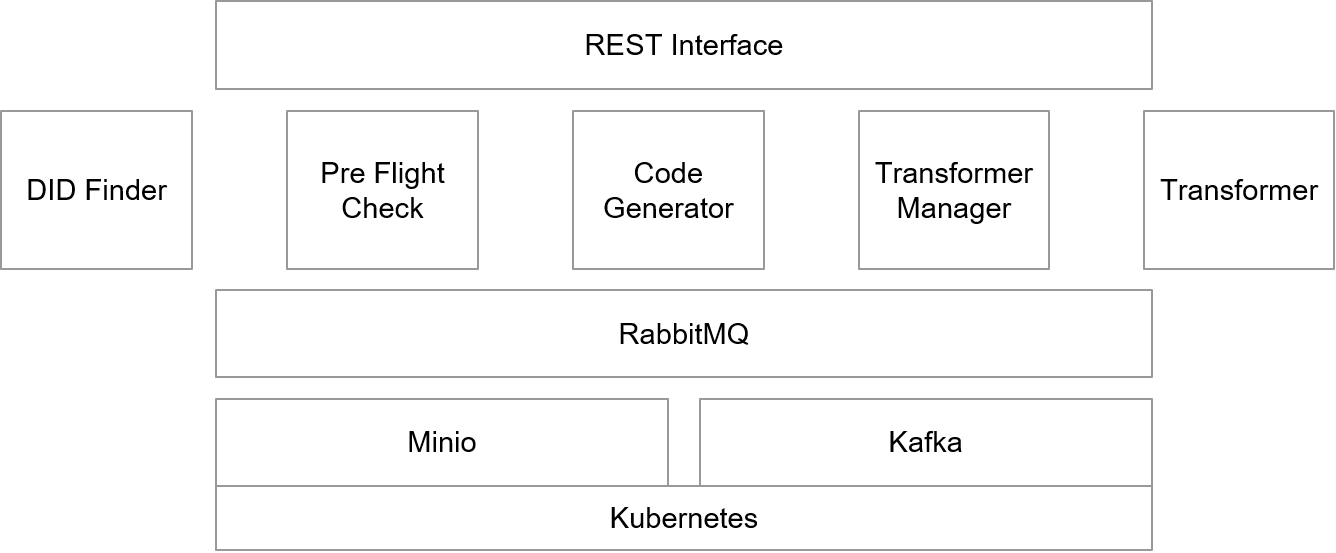
\includegraphics[width=0.75\textwidth]{architectureV2}
  \caption{Architecture for ServiceX version 2, expected to be available in January 2020.}
  \label{fig:architectureV2}
\end{figure}

\subsection{Selection code}
\label{subsec:select}

An example of a typical selection statement is shown below.

\bigskip

{\raggedright \footnotesize
  \texttt{xAOD.Where(}

  \texttt{\quad lambda e: }

  \texttt{\quad \quad e.jet\_pT.Where(lambda pT: }

  \texttt{\quad \quad pT > 1000).Count() > 0)}

  \texttt{\quad .Select('lambda e: }

  \texttt{\quad \quad [e.eventNumber, e.CalibJet\_pT]'}

  \texttt{)}
}

\bigskip

This statement will extract the event number and calibrated transverse momenta of all jets in the
event, provided there is at least one jet in the event with an uncalibrated transverse momentum
greater than 1 GeV.

%
% BibTeX or Biber users please use (the style is already called in the class, ensure that the "woc.bst" style is in your local directory)
% \bibliography{name or your bibliography database}
%
% Non-BibTeX users please use
%
\begin{thebibliography}{}
%
% and use \bibitem to create references.
%
% \bibitem{RefJ}
% Format for Journal Reference: Journal Author, Journal \textbf{Volume}, page numbers (year)
% \bibitem{RefB}
% Format for books: Book Author, \textit{Book title} (Publisher, place, year) page numbers
\bibitem{RefServiceX}
\textit{https://github.com/ssl-hep/ServiceX}
\bibitem{RefEventStreams}
\textit{https://ibm.github.io/event-streams/about/key-concepts/}
\bibitem{uproot}
\textit{https://github.com/scikit-hep/uproot}
\end{thebibliography}

\end{document}

% end of file template.tex

<div id='footer'><table width='100%'><tr><td class='right'><a href='http://fusioninventory.org/'><span class='copyright'>FusionInventory 9.1+1.0 | copyleft <img src='/glpi/plugins/fusioninventory/pics/copyleft.png'/>  2010-2016 by FusionInventory Team</span></a></td></tr></table></div>
